\section{Recommended Software Patterns in SST}
The following patterns can be considered appropriate to implement in the project:
\begin{enumerate}
  \item Façade pattern
  \item Interpreter pattern
\end{enumerate}

\subsection{Façade Pattern}
The current method for a Client to interface the library is to create a derived class of Component and override its methods. While this approach provides extensive control over the functionality of crucial methods such as \texttt{void setup(unsigned int)}, \texttt{void finish(unsigned int)} and \texttt{bool tick(SST::Cycle\_t)}, it requires the Client to have extensive knowledge of the subsystems in the framework. The aforementioned methods, if overridden by the Client, must be implemented properly for the model and the simulation to be functional.

Listing \ref{currentModel} is an interface of a simple Component that simulates a primitive full adder hardware unit.

\begin{figure}[h]
  \caption{Circuit Design of a Simple Full Adder}
  \centering
  
\includegraphics[width=0.6\textwidth]{circuit.png}
\end{figure}

\newpage
\begin{lstlisting}[style=customC++,label=currentModel,caption=Example Interface of an SST Component Model]
#include <sst/core/component.h>
#include <sst/core/interfaces/stringEvent.h>
#include <sst/core/link.h>

class FullAdder : public SST::Component {
public:
  // register and manually configure each of the SST::Links
  // to their corresponding event handlers
  FullAdder(SST::ComponentId_t id, SST::Params& params);

  // implement logic for the model when it is being loaded into
  // the simulation
  void setup() override;

  // implement logic for the model when it is being unloaded from
  // the simulation
  void finish() override;

  // implement logic for the model on every clock cycle in the
  // simulation
  bool tick(SST::Cycle_t cycle);

  // event handlers for all the member SST::Link attributes
  void handle_A(SST::Event* event);
  void handle_B(SST::Event* event);
  void handle_C_in(SST::Event* event);

  // register the component
  SST_ELI_REGISTER_COMPONENT(
    FullAdder, // class
    "fulladder", // element library
    "fulladder", // component
    SST_ELI_ELEMENT_VERSION(1, 0, 0),
    "SST example model",
    COMPONENT_CATEGORY_UNCATEGORIZED)

  // port name, description, event type
  SST_ELI_DOCUMENT_PORTS(
    {"A", "Operand 1", {"sst.Interfaces.StringEvent"}},
    {"B", "Operand 2", {"sst.Interfaces.StringEvent"}},
    {"C_in", "Carry-in", {"sst.Interfaces.StringEvent"}},
    {"S", "Sum", {"sst.Interfaces.StringEvent"}},
    {"C_out", "Carry-out", {"sst.Interfaces.StringEvent"}})

private:
  std::string clock;  // SST parameters
  // SST links
  SST::Link *A_link, *B_link, *C_in_link, *S_link, *C_out_link;
  // other attributes
  std::string A, B, C_in;
  SST::Output output;
};
\end{lstlisting}
\newpage

This Component is a relatively simple example of a model that can be simulated in the SST framework. The hardware logic for the full adder will be implemented in the tick function, where the output values (\texttt{S} and \texttt{C\_out}) are evaluated using the member attributes \texttt{A}, \texttt{B}, and \texttt{C\_in} after they are processed by their corresponding handlers.

Exposing all the complexity of the base methods to the Client can lead to many potential issues. One way to reduce the chances of such issues is to abstract away the steps and methods from the Client using a Facade design pattern. The library, in its current state, does not provide a method to call any of the constructors of the Simulation objects, such as Components and SubComponents. Execution of such objects is done through various command line tools. Even testing of the classes appear to be done through external tools and Python interpreters, which compare the outputs to the expected outputs rather than using asserts.

The following listing is a potential interface that may be possible with the integration of a Facade object into the project.


\begin{figure}[h]
  \caption{Potential Implementation of the Facade Pattern}
  \centering
  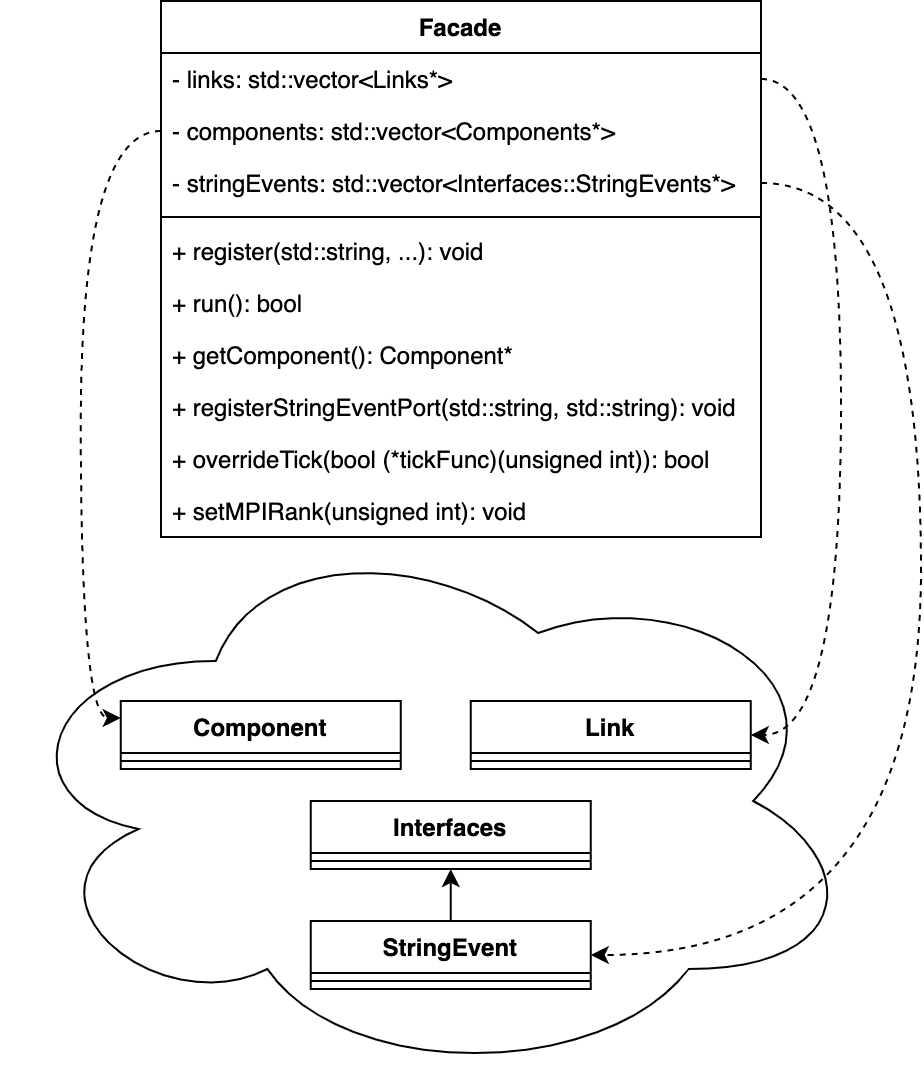
\includegraphics[width=0.8\textwidth]{facade.png}
\end{figure}


\begin{lstlisting}[style=customC++,label=facade,caption=Potential Implementation of Facade]
SST::Facade* facade = new SST::Facade(argc, argv);
SST::Component* component = facade->getComponent();

component->register(
  "FullAdder", // class name
  "fulladder", // element library
  "fulladder", // component
  "1.0.0",
  "SST parent model");
component->registerStringEventPort("A", "Operand 1");
...

component->overrideTick(&customTickFunc);
component->setMPIRank(0);
component->run();

delete component;
delete facade;
\end{lstlisting}

\newpage
\subsection{Interpreter Pattern}
SST requires external Python scripts to configure and run the Client models. The configuration file provides a vast amount of options; from setting the duration of the simulation to providing custom parameters to the models. The configuration file is imported by the provided executables and parsed by the \texttt{Model::Python} classes. The classes map the parameterized method calls made in the configuration file to the implemented class methods.

This method of interpreting the configuration file to generate SST Components for its simulation requires the usage of a Python interpreter. This external dependency potentially adds unnecessary overhead that can be circumvented by integrating the Interpreter pattern into the project. Adding an AbstractExpression class in native C++ will allow the project to not have to rely on an external framework and language to run its simulations.

Instead of a Python script, the simulation configuration can be represented in an XML format. XML parsing is a fairly common task in commercial software that is often achieved by external libraries. Configuration options in SST may require a very simple parser. The AbstractExpression class will perform a similar role to the current \texttt{Model::Python} classes and create SST Components for the simulation.

The following listing is an example of a configuration file for the preceding FullAdder model.
\begin{lstlisting}[style=customPython,label=runPy,caption=Example SST Configuration File \\ File: run.py]
import sst

sst.setProgramOption("stopAtCycle", "5s")

full_add_0 = sst.Component("Full Adder 0", "fulladder.fulladder")
full_add_0.addParams({"clock": "1Hz"})

full_add_1 = sst.Component("Full Adder 1", "fulladder.fulladder")
full_add_1.addParams({"clock": "1Hz"})

full_add_2 = sst.Component("Full Adder 2", "fulladder.fulladder")
full_add_2.addParams({"clock": "1Hz"})

full_add_3 = sst.Component("Full Adder 3", "fulladder.fulladder")
full_add_3.addParams({"clock": "1Hz"})

sst.Link("C_out0").connect(
    (full_add_0, "C_out0", "1ps"),
    (full_add_1, "C_in1", "1ps")
)
sst.Link("C_out1").connect(
    (full_add_1, "C_out1", "1ps"),
    (full_add_2, "C_in2", "1ps")
)
sst.Link("C_out2").connect(
    (full_add_2, "C_out2", "1ps"),
    (full_add_3, "C_in3", "1ps")
)
\end{lstlisting}

The following listing is a potential translation of the preceding configuration file.
\begin{lstlisting}[style=customXML,label=xml,caption=Potential Implementation of an SST Configuration File \\ File: run.xml]
<? xml version="1.0" encoding="UTF-8"?>
<config>
  <setProgramOption stopAtCycle="5s"/><setProgramOption/>
  <component id="full_add_0" name="Full Adder 0" class="fulladder"/>
    <param key="clock" value="1Hz"/><param/>
    <link from="C_out0" to="full_add_1" port="C_in1"/></link>
  <component/>
  <component id="full_add_1" name="Full Adder 1" class="fulladder"/>
    <param key="clock" value="1Hz"/><param/>
    <link from="C_out1" to="full_add_2" port="C_in2"/></link>
  <component/>
  <component id="full_add_2" name="Full Adder 2" class="fulladder"/>
    <param key="clock" value="1Hz"/><param/>
    <link from="C_out2" to="full_add_3" port="C_in3"/></link>
  <component/>
  <component id="full_add_3" name="Full Adder 3" class="fulladder"/>
    <param key="clock" value="1Hz"/><param/>
  <component/>
</config>
\end{lstlisting}

\subsection{Other Minor Idioms}
The project can be found with several \texttt{goto} statements within the code base. The use of this unconditional jump is highly discouraged in the C++ community, although its usage is not considered a part of any idioms. Regardless, the project would benefit from discarding these statements and replacing them with proper conditional jumps for increased clarity and understanding of the project.
